
\section{Results}

??? screenshots of spatial patterns ???
!!! Figure captions !!!
!!! Confidence intervals !!!
!!! ``Code is in the appendix'' !!!

\subsection{Effect of spatial structure in PD and HD games}

In our first simulation experiment, we compared the effect of spatial structure on the persistence of cooperators in the PD and HD games. For the PD game we were able to reproduce the theoretical prediction that spatial structure enables cooperators to persist, even if cooperation is not an evolutionarily stable strategy in well-mixed populations. Our simulated spatial PD population with neighborhood size $= 8$ could maintain an average of $66.5\%$ cooperators ($\pm 1.12 \%$) at a cost-benefit ratio of $r = 0.05$. For higher cost-benefit ratios, however, cooperation was not evolutionarily stable at this neighborhood size and ceased within the 5000 time steps. If cooperation did was cost-free, the proportion of cooperators remained close to its initial value. See figure \ref{fig: task1_4plot} for a comparison of the frequency of cooperation in spatial and nonspatial PD games.


%higher resolution of r values and different nb sizes see next subsection.


\begin{figure}[H]
	\centering 
	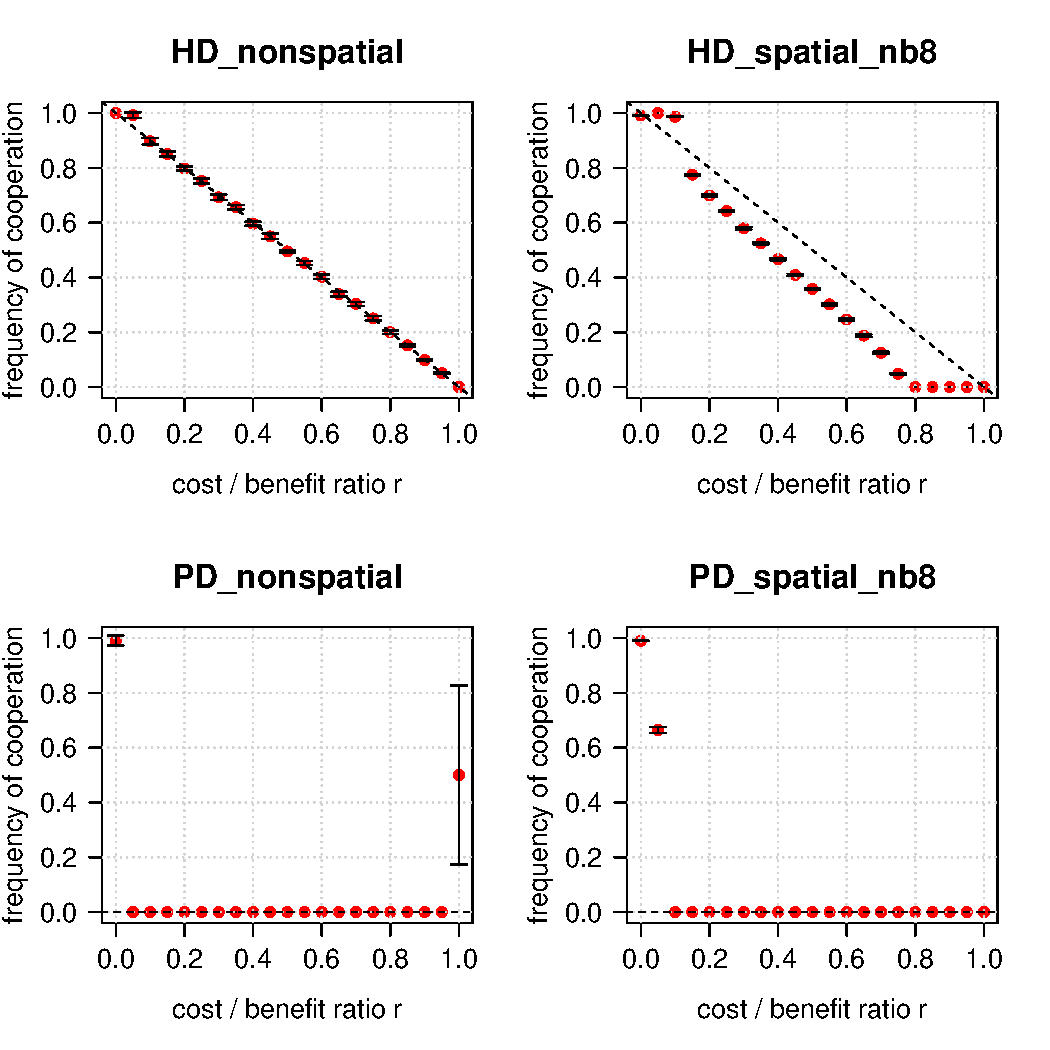
\includegraphics[width=9.5cm]{task1_4plot}
	\caption{Comparison of HD and PD game simulations, both with and without spatial structure.  \textbf{[ t = 5000, i = 10 ]} }\label{fig: task1_4plot}
\end{figure}

In the spatial HD game we found a quite contrary effect of spatial structure. When simulating a well-mixed population we could reproduce the theoretical prediction that the equilibrium frequency of cooperators is $1 - r$. However, adding spatial structure to the model reduced the frequency of cooperators as compared to the non-spatial version for most r values (figure \ref{fig: task1_4plot}). The higher the r value, the bigger the relative disadvantage of cooperators was. For $r \geq 0.8$ cooperation completely vanished from the population. Only at very low cost-benefit ratios, cooperators in the HD game profited from spatial structure. The threshold r value up to which cooperators profited was 0.1 for a neighborhood size of 8.



\subsection{Effect of neighbourhood size}

In the second simulation experiment we varied neighborhood size in the spatial PD and HD games and investigated whether changes in neighborhood size would change the effects of spatiality. Except for neighborhood size, the HD simulations were run with the exact same parameter set as before. In the first PD game simulation spatial structure only came into effect at very small r-values. To achieve a reasonably high x-axis resolution in the most relevant section, we lowered the r-stepwidth from $0.05$ to $0.01$ for r-values $< 0.1$ in the second PD experiment.
% Move last two sentences to figure caption?

\subsubsection*{Spatial HD games}
Varying neighborhood size in the HD game yielded three main observations:\\ 
In the spatial HD game with eight neighbors, cooperators profited from spatial structure at low cost-benefit ratios and suffered at higher r-values. This also goes for different neighborhood sizes. However, the threshold r-value at which benefit turns into disadvantage varies with neighborhood size: It is higher for small neighborhood sizes and decreases with increasing neighborhood size.\\
In addition to the increased benefit from spatial structure at small r-values, smaller neighborhood sizes (4 neighbors) had another effect in the second HD experiment: The detriment of spatial structure in comparison to well-mixed populations increased faster for r-values above the threshold r-value. In contrast, bigger neighborhoods ($>8$ neighbors) were less detrimental to cooperators at high r-values.\\
At the upper end of the range of r-values, another effect of neighborhood size became apparent: The r-value above which total extinction of cooperators becomes likely changed with neighborhood size. The smaller the neighborhood, the more likely cooperators are to die out completely. With $N$ being the average number of neighbors, cooperators were likely to die out completely if $1 / N > 1 - r$. The effects of varying neighborhood sizes in the HD game are illustrated in figure \ref{fig: task2_4plot}.\\


\begin{figure}[H]
	\centering 
	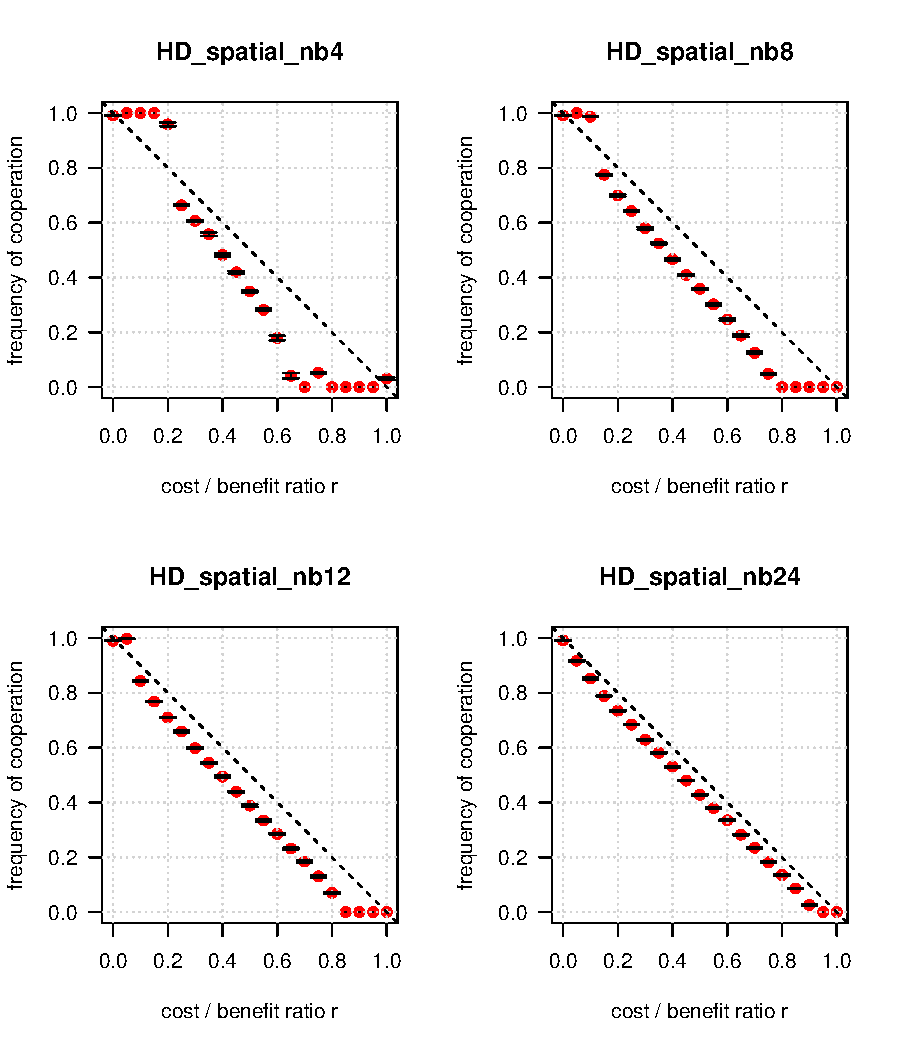
\includegraphics[width=9.5cm]{task2_4plot}
	\caption{Effect of varying neighborhood size in the HD game.  \textbf{[ t = 5000, i = 10 ]} }\label{fig: task2_4plot}
\end{figure}



\subsubsection*{Spatial PD games}





\begin{figure}[H]
	\centering 
	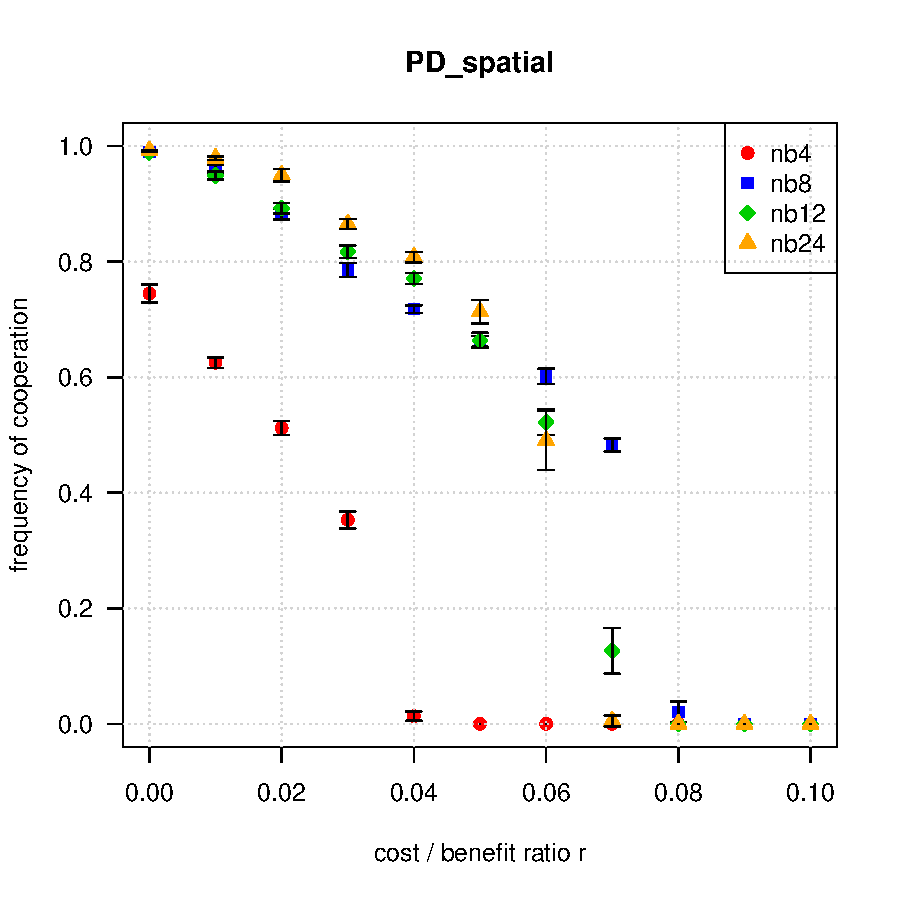
\includegraphics[width=9.5cm]{task2_multiplot}
	\caption{Spatial PD game simulations with different neighborhood sizes.  \textbf{[ t = 5000, i = 10 ]} }\label{fig: task2_multiplot}
\end{figure}


It is widely assumed that spatial structure allows for the evolution of cooperation in PD games. However, this goes only for a small range of cost-benefit ratios. Cooperation is only evolutionarily stable for r-values $ \leq 0.09$, for bigger r-values it disappears from the population.\\
 
In spatial HD games: small neighborhoods = bigger profit when r is small, and small neighborhoods = bigger disadvantage when r is big.

In spatial PD games: 

Found anomality

r 0.03, nb4 -> stable at propC 0.35 after 2500 steps -> stable
r 0.065, nb4 -> cooperators die after 900 steps -> unstable
r 0.03, nb8 -> stable at propC 0.77 after 10000 steps -> stable
r 0.065, nb8 -> stable at propC 0.55 after 2500 steps -> stable
r 0.03, nb12 -> stable at propC 0.825 after 7500 steps -> stable
r 0.065, nb12 -> randomly oscillating around propC 0.33 after 10000 steps -> half-stable
r 0.03, nb24 -> stable at propC 0.85 after 4000 steps -> stable
r 0.065, nb 24 -> cooperators die after 7400 steps -> unstable

\begin{itemize}
\item{\textbf{spatial structure does not automatically make a system stable}}\\
\item{\textbf{two variables influence whether a system is stable: neighborhood size and cost-benefit ratio}}
\end{itemize}



fixed r: at 0.03 and 0.065
varying neighborhood size
5000 steps, 5 repetitions

\begin{figure}[H]
	\centering 
	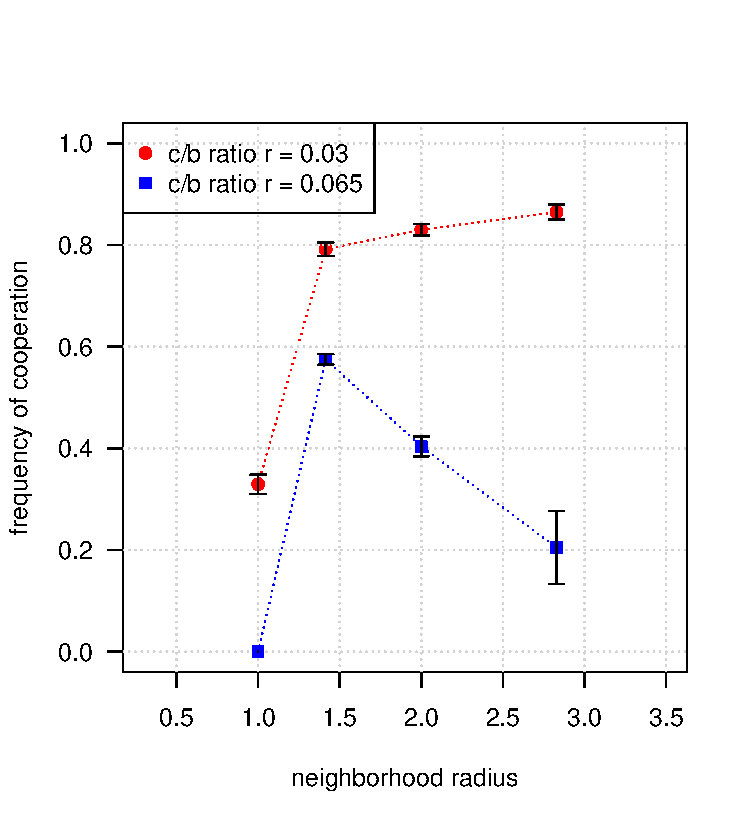
\includegraphics[width=9.5cm]{task2_radiusplot}
	\caption{Spatial PD game simulations with fixed cost-benefit-ratio and different neighborhood sizes. Radius 1 is adequate to 4 neighbors, radius 1.4 = 8 neighbors, radius 2 = 12 neighbors and radius 2.8 = 24 neighbors.  \textbf{[ t = 10000, i = 10 ]} }\label{fig: task2_radiusplot}
\end{figure}


\subsection{Effect of mixed strategies}

In our third experiment, we compared the effect of spatial structure in the mixed-strategy HD game with that in the pure-strategy game.


\begin{figure}[H]
	\centering 
	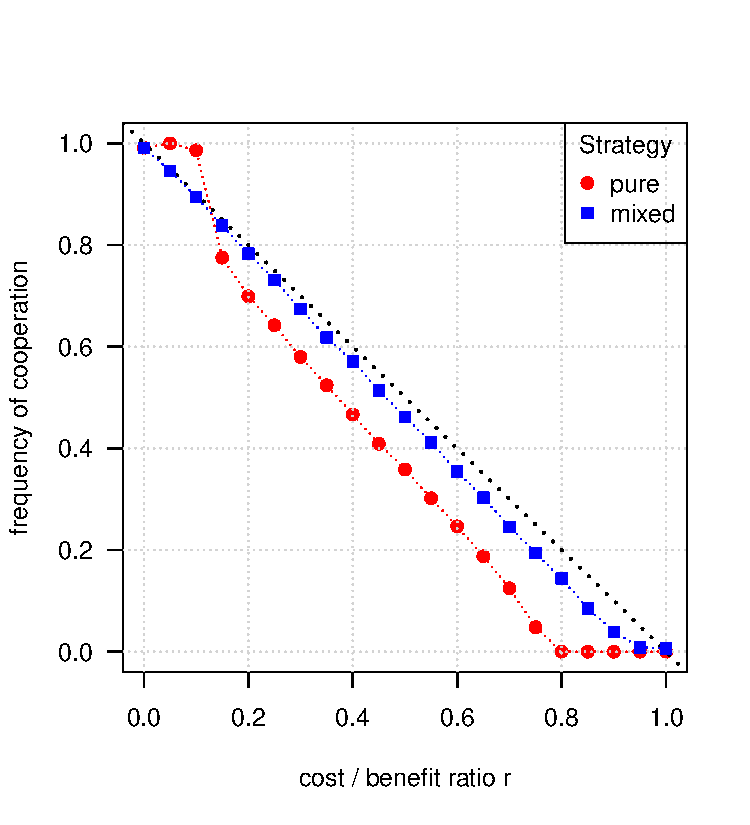
\includegraphics[width=9.5cm]{task3_multiplot}
	\caption{Spatial HD game simulations with neighborhood size 8 and different strategies. The dotted black line depicts the frequency of cooperation in nonspatial games.  \textbf{[ t = 10000, i = 10 ]} }\label{fig: task3_multiplot}
\end{figure}





